\subsection{Orbit Closure \label{sec:03_OrbitClosure}}



%%%%%%%%%%%%%%%%%%%%%%%%%%%%%%%%%%%%%%%%%%%%%%%%%%%%%%%%%%%%%%%%%
\subsubsection{Horizontal and vertical orbit matching}
%

Unfortunately the BPMs installed at CTF3 could not resolve the single bunch orbit, 
and it was impossible to observe directly the orbit mismatch between recombined bunches.
In case of the Delay Loop the orbit mismatch measurement was done with a pulse 
for which the first half of the train bypassed the DL, while the second half was delayed.
Than the two subpulses followed each other in TL1 and CR separated by a gap corresponding to 
the Delay Loop time of flight. It required a 280 ns-long 1.5~GHz bunch train.
The phase of the bunches had to be flipped by 180 degrees with respect to the nominal setup.
This way the second half of the train was injected to the Delay Loop instead of the first half. 
Hence, rather then combining the two sub-trains of bunches, they were separated from each other and 
their orbit difference was easily measured in the following transfer line.
Unfortunately this technique had two main disadvantages:
%
\begin{itemize}
\item
In order to perform the measurement and correction a dedicated beam had to be set-up
starting from the injector.
This meant that the measured orbit difference might not be the actual mismatch that was in
place during the factor-2 recombination.
\item
The BPMs installed in the TL1 transfer line were known to misbehave with such a beam,
providing inconsistent performances between the measurement of the delayed and bypassing
bunches. This issue is not yet fully understood.
\end{itemize}
%

In order to avoid these issues a simpler set-up was used.
The target orbit in TL1 was measured by using the nominal 1.5~GHz beam, but forcing it to
bypass the DL by switching off the RF deflector and replacing its function with two orbit corrector magnets.
This was a standard procedure to bypass the DL independently of the kind of beam that is
produced in the linac.
Afterwards the beam was magnetically injected and extracted from the DL, and its orbit in
TL1 was corrected by acting only on the correctors inside the DL. 
The magnetic injection makes use of the same correctors used to magnetically bypass the DL,
but with opposite kick.

Figure~\ref{fig:orbitCorrectionDLmatching} shows an example of horizontal~\subref{fig:orbitCorrectionDLmatchingH} and vertical~\subref{fig:orbitCorrectionDLmatchingV} orbit corrections achieved in the latest
CTF3 run of 2015.
For these corrections the variation of the DL corrector strengths is shown in
Figure~\ref{fig:correctorsCorrectionDLmatching}.
%
\begin{figure}[htbp]
  \subfloat[Horizontal]{
    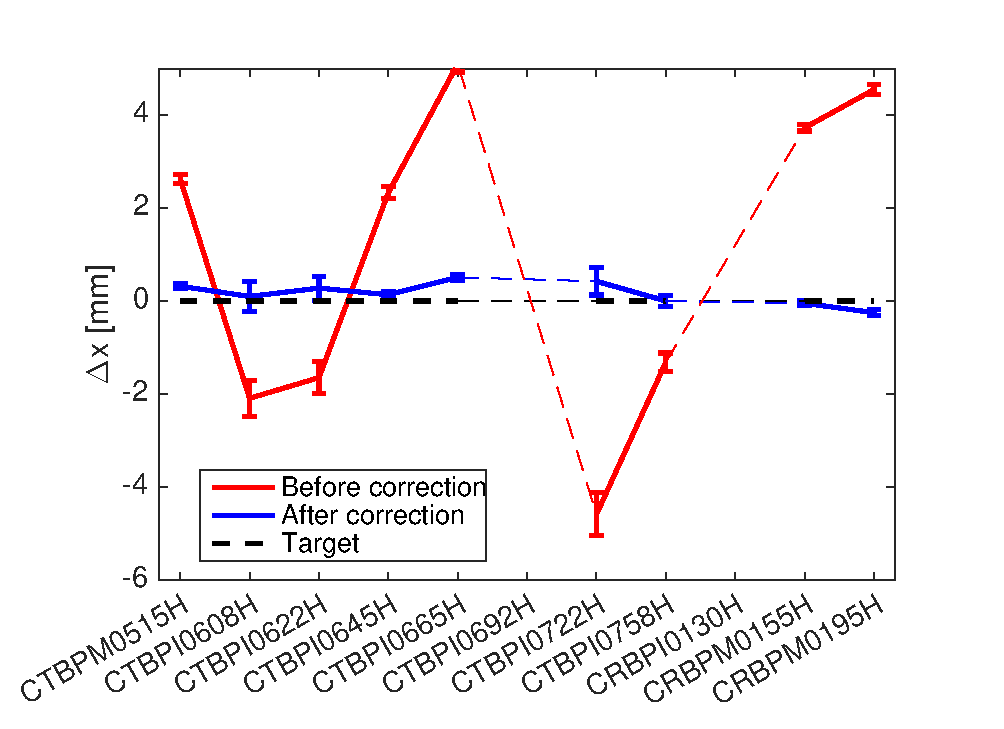
\includegraphics[width=0.45\textwidth]{DLorbitclosureHobservables_delta.eps}
    \label{fig:orbitCorrectionDLmatchingH}
  }
  \qquad
  \subfloat[Vertical]{
    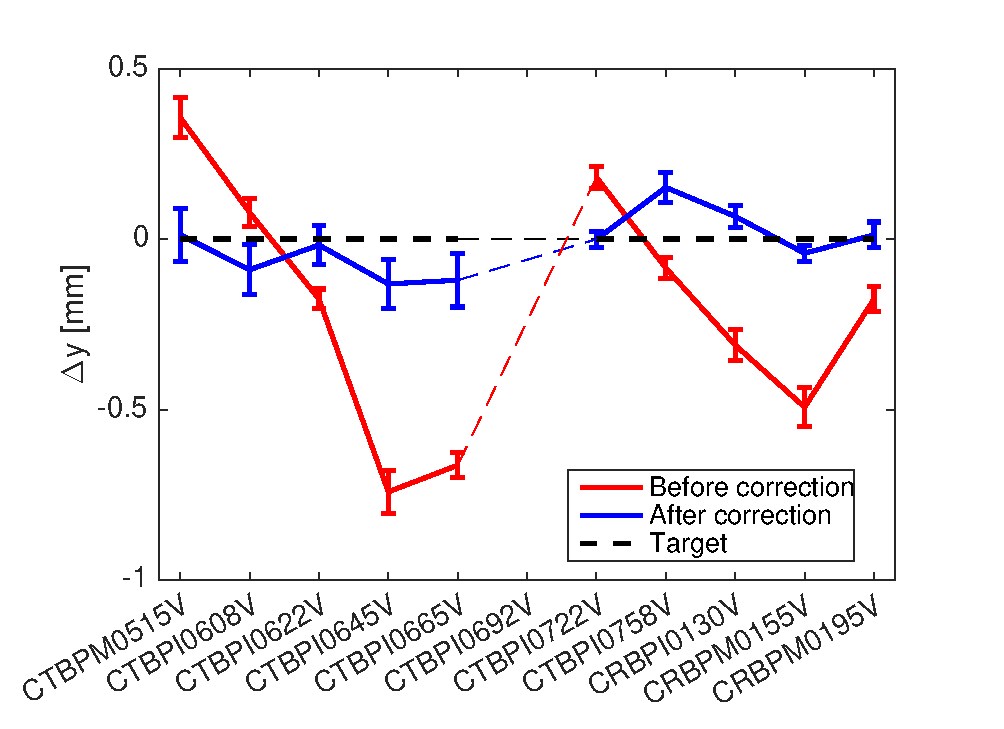
\includegraphics[width=0.45\textwidth]{DLorbitclosureVobservables_delta.eps}
    \label{fig:orbitCorrectionDLmatchingV}
  }
  \caption{Difference between the delayed and bypassing beam orbits in the TL1 BPMs before
           (red) and after (blue) orbit matching correction.
           \protect\subref{fig:orbitCorrectionDLmatchingH}  horizontal plane.
           \protect\subref{fig:orbitCorrectionDLmatchingV} vertical plane.
           The error bars are the statistical error on about 20 orbit measurements.
           The dashed-black lines represent the desired difference that is naturally zero.
           Note that BPM CTBPI0692 was not operational at the time of the experiment, while
           thehorizontal position in BPM CRBPI0130 was not usable due to hardware limitations.
           No values are given in these cases and dashed lines connect the points before and
           after the faulty BPMs.
  }
  \label{fig:orbitCorrectionDLmatching}
\end{figure}
%
%
\begin{figure}[htbp]
\subfloat[Horizontal]{
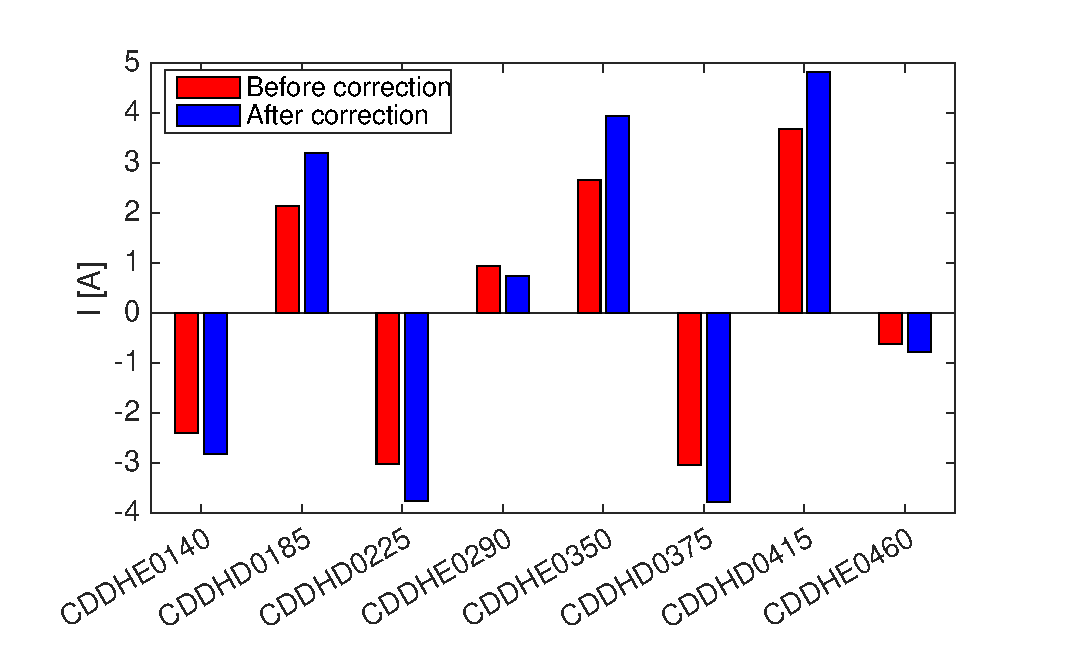
\includegraphics[width=0.45\textwidth]{DLorbitclosureHcorrectors.eps}
\label{fig:correctorsCorrectionDLmatchingH}
}
\qquad
\subfloat[Vertical]{
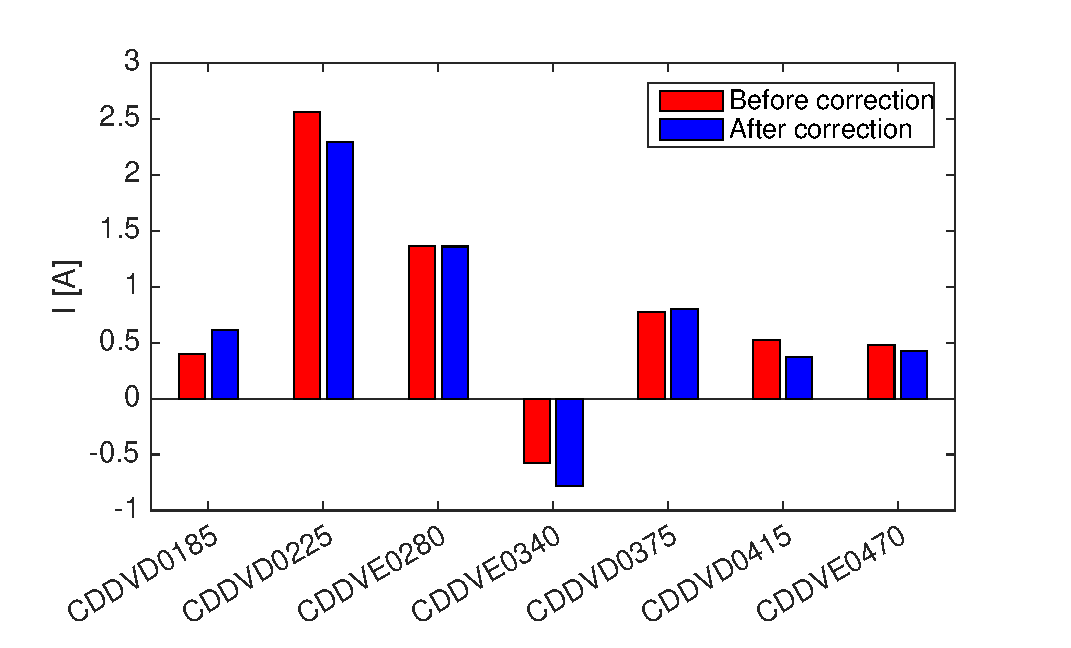
\includegraphics[width=0.45\textwidth]{DLorbitclosureVcorrectors.eps}
\label{fig:correctorsCorrectionDLmatchingV}
}
\caption{DL corrector strengths before (red) and after (blue) the orbit matching in TL1
between the delayed beam and bypassing beam. 
\protect\subref{fig:correctorsCorrectionDLmatchingH} is for to the horizontal plane, while
\protect\subref{fig:correctorsCorrectionDLmatchingV} is for the vertical one.
}
\label{fig:correctorsCorrectionDLmatching}
\end{figure}
%
The final orbit matching obtained in Figure~\ref{fig:orbitCorrectionDLmatching} has to be
compared with the tolerances derived in Section~\ref{sub:monochEffDL} and presented in
Figure~\ref{fig:orbitTolTL1}.
For both planes, if one trusts the calibrations of the BPMs, after the correction the
expected projected emittance growth is below 50\% for both definitions of emittance
presented in Section~\ref{sub:noteSimulEmit}.
A better correction appears to be challenging with the aperture constraints of the DL.
However such an emittance growth can be acceptable.

It is interesting to note in
Figure~\ref{fig:correctorsCorrectionDLmatching}\subref{fig:correctorsCorrectionDLmatchingH}
that the DL correctors are fired in an alternating pattern.
The linearFeedback application used for the correction is normally able to remove
unnecessary correction by targeting a proper correctors pattern, 
e.g. all the correctors with null strength.
Unfortunately the dynamic aperture of the DBRC at CTF3 and in particular of the DL does not
allow much freedom.
For this reason most of the corrections presented in this chapter are not targeting a null
strength on the correctors, but rather the initial corrector strengths that were
empirically found by optimising beam transmission.
However
Figure~\ref{fig:correctorsCorrectionDLmatching}\subref{fig:correctorsCorrectionDLmatchingH}
suggests that the bending magnets of the DL could have been wrongly set with respect to the
beam energy, and hence the correctors are compensating for this error.
A possible improvement of the correction could then be to use not only the correctors, but
also the strengths of the bending magnets. %, as steerers.



The next step in the beam recombination process at CTF3 is the factor-4 recombination that 
takes place in the Combiner Ring (CR).
Here a set of measurements and corrections with the aim of improving the quality of 
a pure factor-4 recombination in the CR are reported.
This means that all the results presented in this section have been obtained with 
a beam that was bypassing the DL using magnetic correctors instead of the RF deflector 
normally used for the factor-2 recombination.
The beam generated from the linac was at 3 GHz, which was then not suitable for 
the full factor-8 recombination.

Note that the reported experiments were not performed in chronological order.
Even in the chronological case, the facility could have been set up for different experiment 
from day to day, so earlier corrections and performance might not be preserved 
between different experiments. 


In the Combiner Ring there were two possibilities to inject the beam into the closed orbit:
\begin{itemize}
\item Modify the incoming orbit such that the beam is injected onto 
      the natural closed orbit of the ring.
\item Modify the closed orbit of the ring by acting on the correctors installed in 
      the ring itself, and so match the closed orbit of the ring with the incoming orbit.
\end{itemize}
%
The first method is probably the cleanest: 
one could measure the closed orbit of the ring by taking the average orbit of 
a beam circulating for many turns, hence steer the incoming beam such that 
the first turn orbit equals the closed orbit previously measured.
On the other hand this requires one to have a beam already circulating for many turns 
into the ring, and have BPMs able to measure precisely the orbit for several turns.
Normally this is not the case at CTF3. From experience at CTF3 it turns out that the most effective
approach is the second one. The orbit closure correction was performed by acting on the correctors of
the CR while minimising the difference between the orbits of the first and second turns in the ring.

Figure \ref{fig:orbitCRmatchingMeas} shows an example of such a correction.
Not all the BPMs of the CR were used, but only those in dispersion-free areas of the ring. 
This was an attempt to minimise the energy effects observed in BPMs that are normally in 
regions with high dispersion.
%
\begin{figure}[htbp]
\centering
\subfloat[Horizontal]{
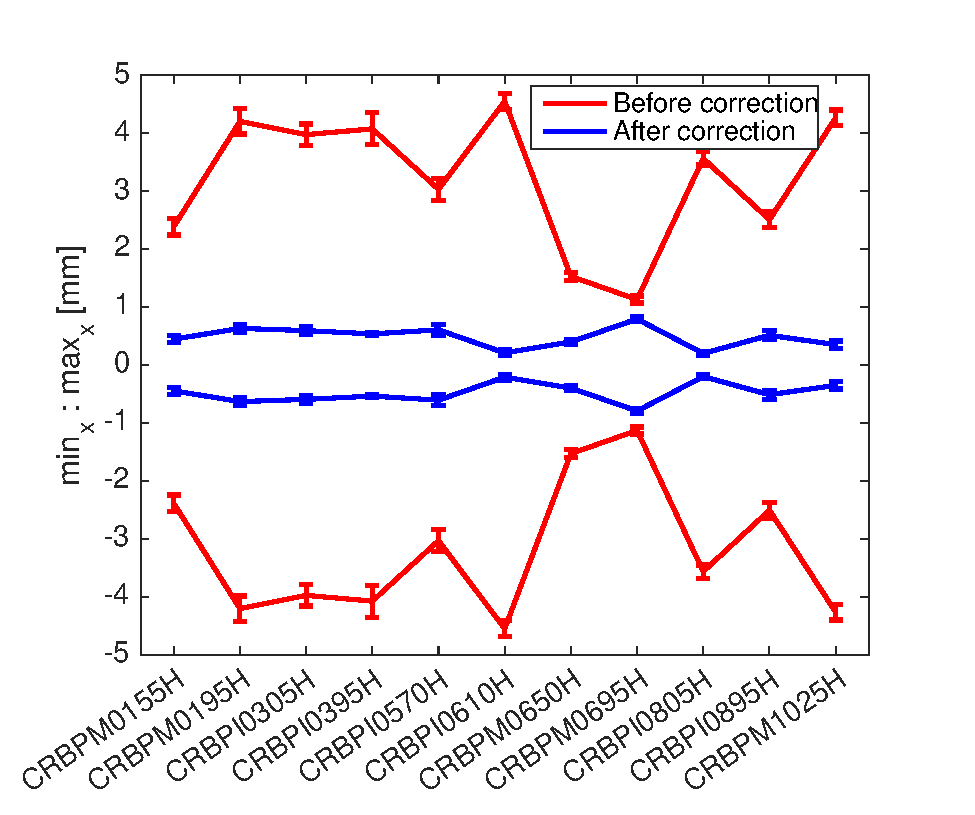
\includegraphics[width=0.45\textwidth]{CRoCloseH_corridorBeforeAfter.eps}
\label{fig:orbitCRmatchingMeasH}
}
\qquad
\subfloat[Vertical]{
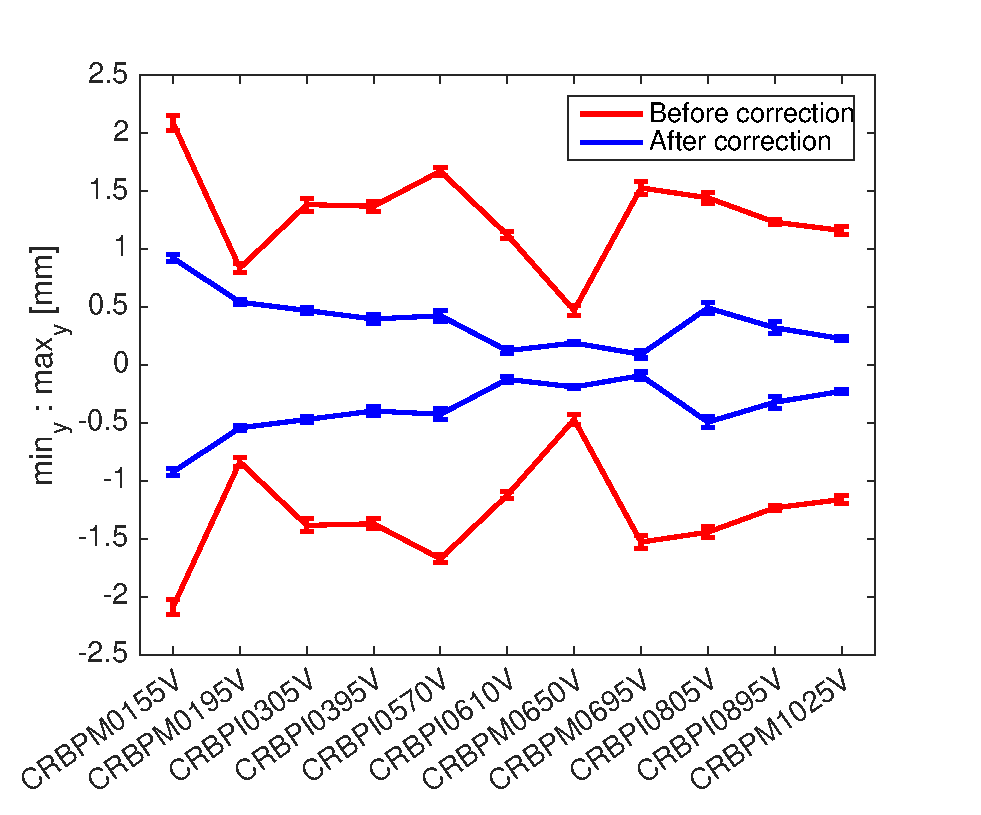
\includegraphics[width=0.45\textwidth]{CRoCloseV_corridorBeforeAfter.eps}
\label{fig:orbitCRmatchingMeasV}
}
\caption{Horizontal~\protect\subref{fig:orbitCRmatchingMeasH} and 
         vertical~\protect\subref{fig:orbitCRmatchingMeasV} orbit corridors within which
         the orbit of a beam circulating for 4 turns in the CR are confined before (red) and 
         after (blue) an orbit closure correction.}
\label{fig:orbitCRmatchingMeas}
\end{figure}
%
The strengths of the correctors that were used for the correction 
are shown in Figure~\ref{fig:orbitCRmatchingCorr}.
For the vertical plane it is important to point out that the feedback tool 
was able not only to heavily reduce the orbit mismatch, 
but also to remove the unnecessary power of the last three correctors in the ring. 
%
\begin{figure}[bp]
\centering
\subfloat[Horizontal]{
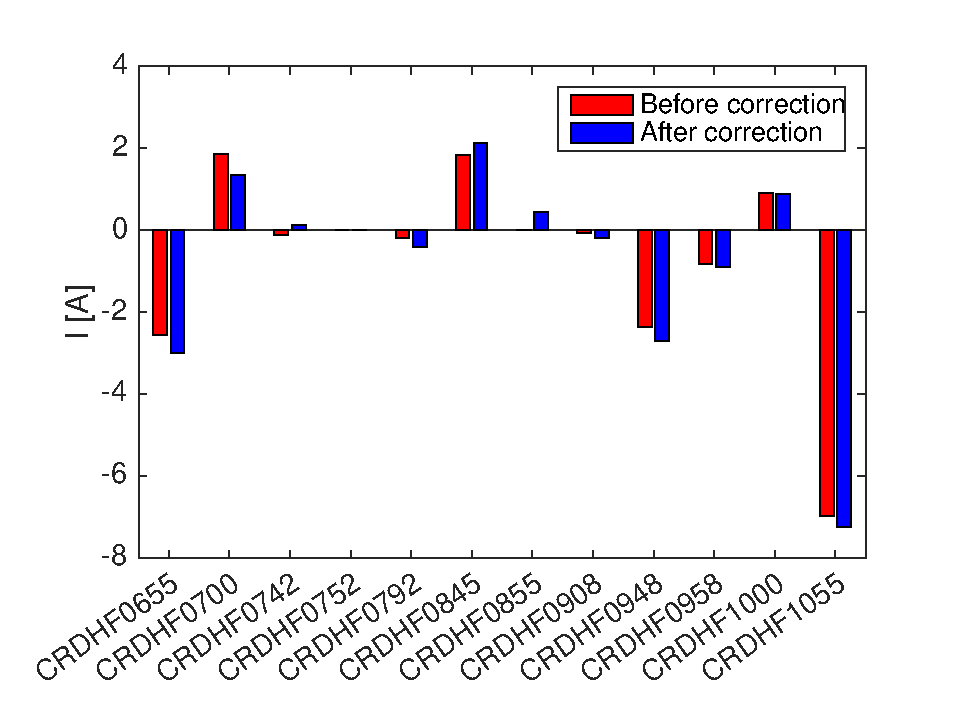
\includegraphics[width=0.45\textwidth]{CRoCloseH_correctors.eps}
\label{fig:orbitCRmatchingCorrH}
}
\qquad
\subfloat[Vertical]{
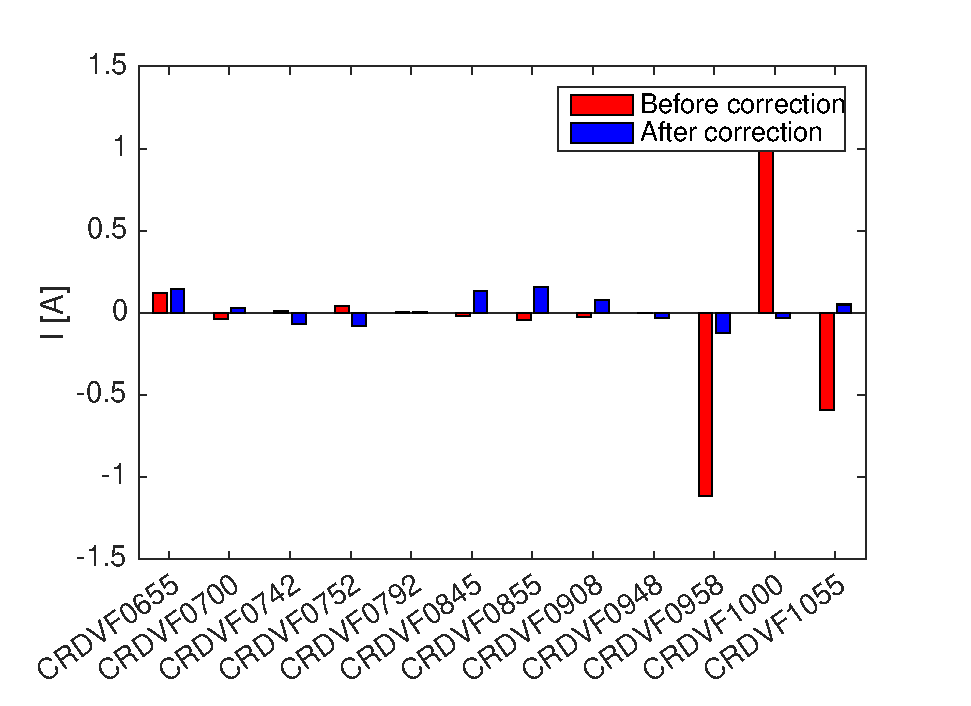
\includegraphics[width=0.45\textwidth]{CRoCloseV_correctors.eps}
\label{fig:orbitCRmatchingCorrV}
}
\caption{Strength of the horizontal~\protect\subref{fig:orbitCRmatchingCorrH} and 
         vertical~\protect\subref{fig:orbitCRmatchingCorrV} correctors in 
         the CR before (red) and after (blue) an orbit closure correction.}
\label{fig:orbitCRmatchingCorr}
\end{figure}
%
At the BPMs shown in Figure~\ref{fig:orbitCRmatchingMeas} the orbit difference between
different turns was reduced to below 1 mm in the horizontal plane and 0.5 mm in the
vertical.
The result obtained should be compared with the tolerances for an ideal machine that
were presented in Section~\ref{subs:crtollerances} (Figure~\ref{fig:orbitTolCR}).
Note that for the vertical plane the statistical emittance growth one should expect
should be below 30\%, while in the horizontal plane things are more critical, being
close to the 70\% envelope of Figure~\ref{fig:orbitTolCR}\subref{fig:orbitTolCRH}.

Unfortunately there was not enough time to systematically measure the initial and final
Twiss parameters of the different turns before and after the orbit correction presented
in Figure~\ref{fig:orbitCRmatchingMeas}.
Only for the vertical plane a measurement of the Twiss parameters of a factor-4
combined beam was taken right before and after the orbit correction presented here,
while for the horizontal plane this measurement was performed only after the orbit
correction.
For the horizontal plane one can consider as a reference the latest measurement
presented in the previous section.
Figure~\ref{fig:orbitCRmatchingQuad} shows the comparison between the beam variance for
the different scans, while the fitted Twiss parameters are reported in
Table~\ref{tab:orbitCRmatchingQuad}.
%
\begin{figure}[b!p]
\centering
\subfloat[Horizontal]{
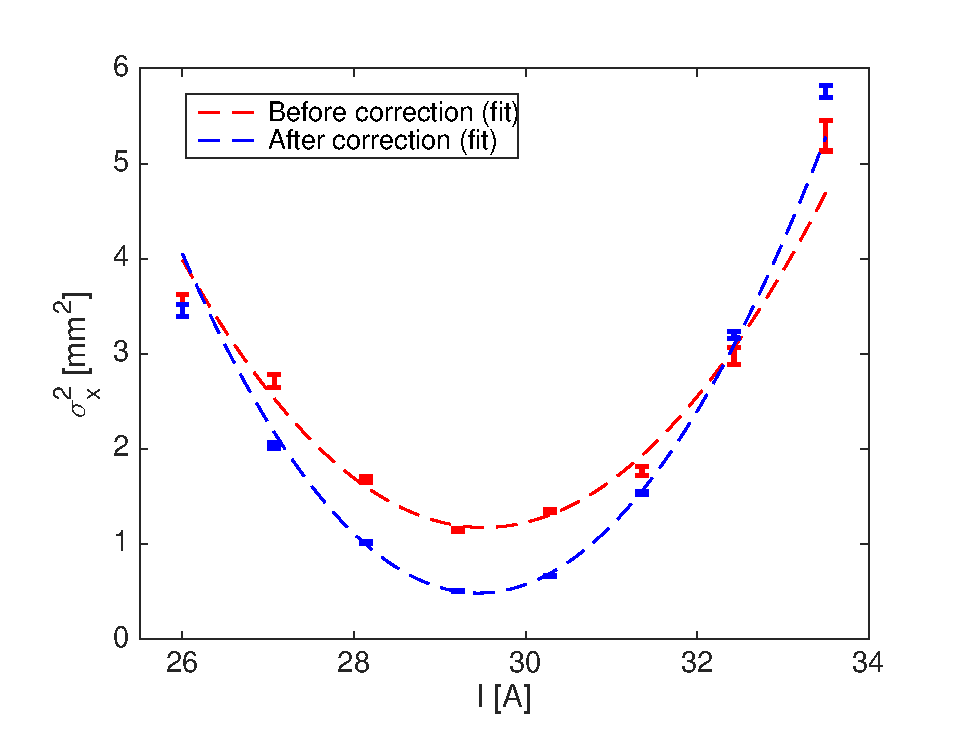
\includegraphics[width=0.45\textwidth]{CRoCloseH_oldBefore_AfterComparisonQuadscan271.eps}
\label{fig:orbitCRmatchingQuadH}
}
\qquad
\subfloat[Vertical]{
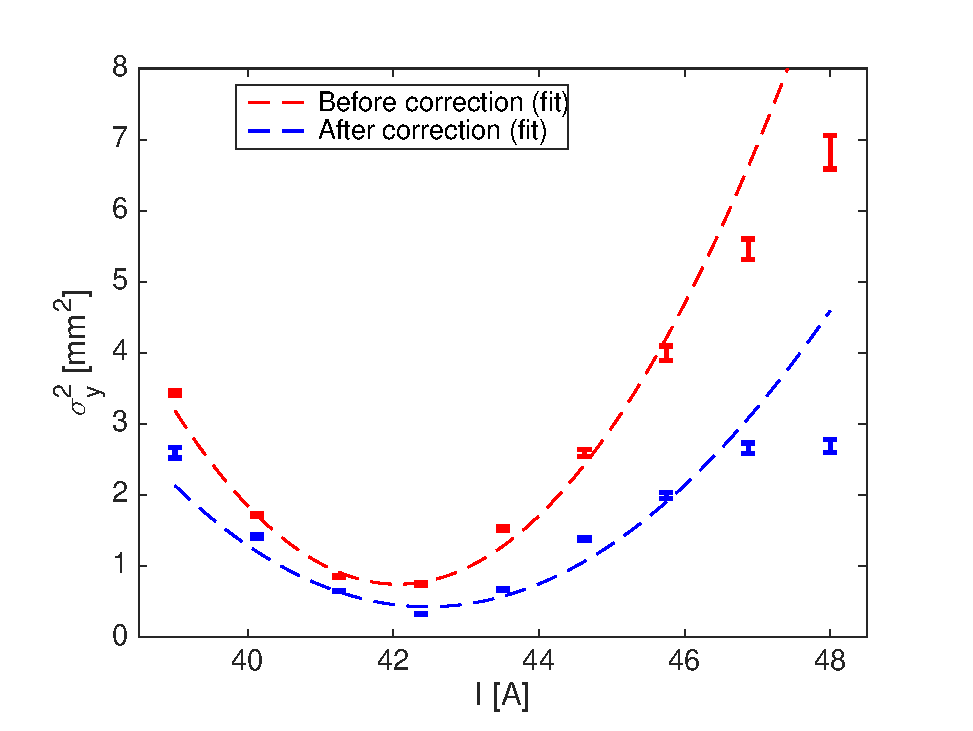
\includegraphics[width=0.45\textwidth]{CRoCloseV_beforeAfterQuadscan271.eps}
\label{fig:orbitCRmatchingQuadV}
}
\caption{Beam variance measured at the screen CC.MTV0253 in TL2 as a function of
         the quadrupole current used to perform quadrupole scan measurements
         in the horizontal \protect\subref{fig:orbitCRmatchingQuadH} and vertical
         \protect\subref{fig:orbitCRmatchingQuadV} plane.
         The red points are relative to a combined factor-4 beam before orbit
         closure correction, while in blue is the same scan after the correction
         presented in Figure~\ref{fig:orbitCRmatchingMeas}.
         The error bars are computed from the Gaussian fits to the profiles
         measured at the screen.
         The dashed lines are the fits to the data corresponding to the Twiss
         parameters that are reported in Table~\ref{tab:orbitCRmatchingQuad}.
         Note that the red scan in the horizontal plane was performed a few days
         before the orbit correction.}
\label{fig:orbitCRmatchingQuad}
\end{figure}
%
%
\begin{table}
\centering
\begin{tabular}{l c c c c c c}
\hline
                     & $\beta_x$  [m]  &  $\alpha_x$     &  $\epsilon_{Nx}$   [$\mu$m]   & $\beta_y$  [m]  &  $\alpha_y$     &  $\epsilon_{Ny}$   [$\mu$m]    \\
\hline
Nominal values       & $8.9$       & $-7.2$       & --             & $4.8$       & $0$       & -- \\
Before correction    & $4.1 \pm 0.4$   & $-2.9 \pm 0.3$   & $234 \pm 9$         & $7.2 \pm 0.7$   & $-1.4 \pm 0.2$   & $66 \pm 3$ \\ 
After correction     & $7.1 \pm 0.3$   & $-5.3 \pm 0.3$   & $173 \pm 4$         & $6.7 \pm 1.3$   & $-1.5 \pm 0.4$   & $37 \pm 3$ \\
\hline
\end{tabular}
\caption{Comparison between Twiss parameters of a factor-4 beam measured at 
         screen CC.MTV0253 before and after orbit closure in the CR.
         Note that for the horizontal plane the measurement was performed 
         a few days before the correction.
}
\label{tab:orbitCRmatchingQuad}
\end{table}
%
In the vertical plane the effect of the orbit correction is clear, and
it results in almost a factor-2 reduction of the overall emittance.
For the horizontal plane, as already stated, no measurement right
before the correction is available, so it is possible that many
parameters could have changed between the quadrupole scan measurements.
Still a 25\% emittance reduction is visible and also the Twiss
parameters $\alpha_x$ and $\beta_x$ seem to get closer to the nominal
values. 

In general one can state that the orbit closure correction brings an
evident benefit in the combined beam quality, which is still believed
to be one of the main source of emittance growth in the CR.









